\documentclass[11pt, a4paper]{article}

% ==========================================
% 宏包调用 (Packages)
% ==========================================
\usepackage[utf8]{inputenc}
\usepackage[T1]{fontenc}
\usepackage{lmodern}
\usepackage{geometry}
\usepackage{hyperref}
\usepackage{graphicx}
\geometry{top=2.5cm, bottom=2.5cm, left=2.5cm, right=2.5cm} % 设置适合 12 页阅读的页边距

% 数学与符号宏包
\usepackage{amsmath, amsthm, amssymb, mathrsfs, mathtools}
\usepackage{hyperref}
\hypersetup{
    colorlinks=true,
    linkcolor=blue,
    filecolor=magenta,      
    urlcolor=cyan,
    citecolor=red,
}

% 绘图宏包 (核心)
\usepackage{tikz}
\usetikzlibrary{calc, math, arrows.meta, backgrounds}
\usetikzlibrary{decorations.pathreplacing}
% ==========================================
% 自定义命令与数学符号 (Custom Commands)
% ==========================================
\newcommand{\R}{\mathbb{R}}
\newcommand{\C}{\mathbb{C}}
\newcommand{\Z}{\mathbb{Z}}
\newcommand{\Q}{\mathbb{Q}}
\newcommand{\HH}{\mathbb{H}} % 上半平面 (避免与通常的 \H 冲突)
\newcommand{\SL}{\mathrm{SL}_2(\Z)}
\newcommand{\PSL}{\mathrm{PSL}_2(\Z)}

% ==========================================
% 定理环境设置 (Theorem Environments)
% ==========================================
\theoremstyle{plain}
\newtheorem{theorem}{Theorem}[section]
\newtheorem{lemma}[theorem]{Lemma}
\newtheorem{proposition}[theorem]{Proposition}
\newtheorem{corollary}[theorem]{Corollary}

\theoremstyle{definition}
\newtheorem{definition}[theorem]{Definition}
\newtheorem{example}[theorem]{Example}

\theoremstyle{remark}
\newtheorem{remark}[theorem]{Remark}

\newtheorem{construction}{Construction}[section]

\title{From Farey Diagrams to Modular Forms: A Geometric Introduction}
\author{}
\date{\today}

\begin{document}

\maketitle
\section{Introduction}
\newpage 

\section{Topology of Fractions: Farey's Diagram}
Let $\infty = 1/0$ and $\hat{\Q}=\Q \cup \{\infty\}$.

\begin{definition}[The Abstract Farey Graph]
The abstract Farey graph $\mathcal{F}$ is a graph defined by the following combinatorial data:
\begin{itemize}
    \item \textbf{Vertices:} The vertex set $V$ is the extended rational numbers $\hat{\Q} = \Q \cup \{\infty\}$. Each rational number is written in its lowest terms as a fraction $\frac{a}{b}$ with $\gcd(a,b)=1$ and $b>0$. The point at infinity is represented formally as $\frac{1}{0}$ (and optionally $\frac{-1}{0}$).
    \item \textbf{Edges:} Two distinct vertices $\frac{a}{b}$ and $\frac{c}{d}$ are connected by an undirected edge if and only if they satisfy the unimodular determinant condition:
    $$|ad - bc| = 1.$$
\end{itemize}
\end{definition}
\begin{figure}[htbp]
    \centering
    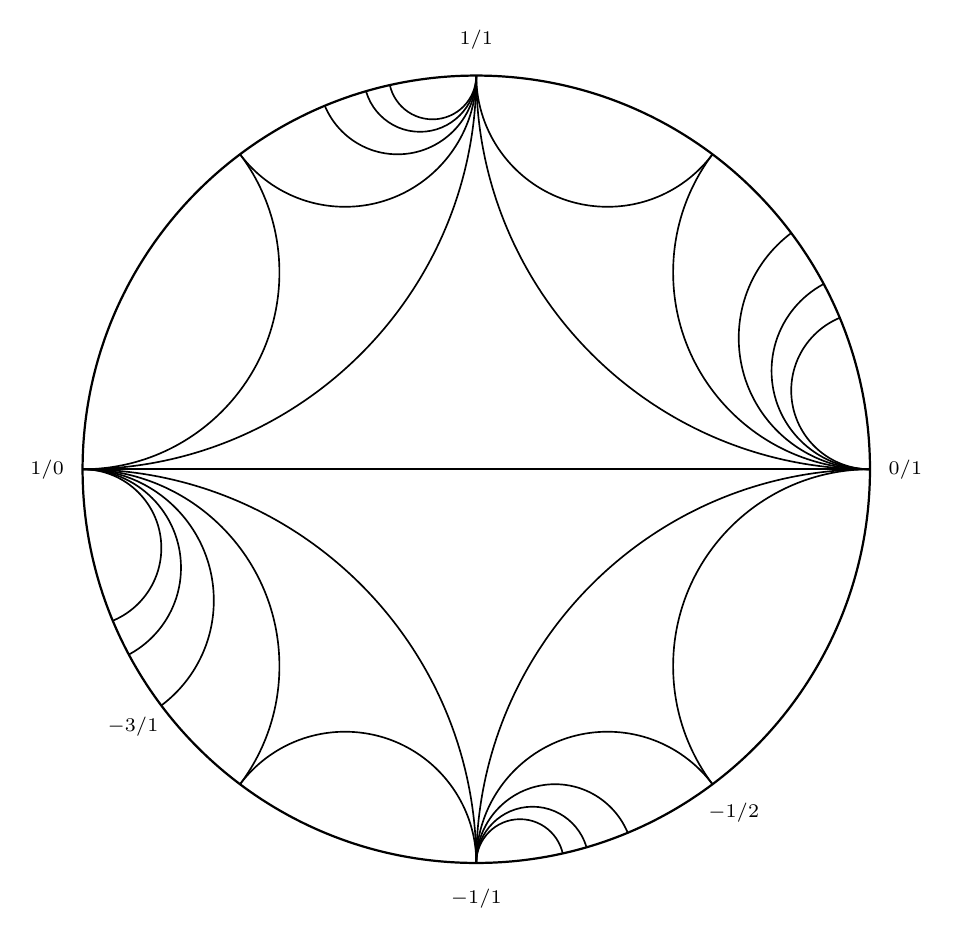
\begin{tikzpicture}[scale=1]
    % 定义圆盘的半径
    \def\R{5}
    
    % --- 宏：计算并绘制分数节点 ---
    \newcommand{\fnode}[2]{
        % 角度变换映射：2 * arctan(y/x)
        \pgfmathsetmacro{\ang}{2*atan2(#1, #2)}
        \node[font=\scriptsize, inner sep=1pt] at (\ang:\R+0.45) {$#1/#2$};
    }
    
    % --- 宏：计算并绘制两条测地线之间的双曲圆弧 ---
    \newcommand{\drawgeodesic}[4]{
        \pgfmathsetmacro{\angA}{2*atan2(#1, #2)}
        \pgfmathsetmacro{\angB}{2*atan2(#3, #4)}
        \pgfmathsetmacro{\diff}{abs(\angA - \angB)}
        
        % 判断是否为穿过圆心的直线（即角度差为 180 度）
        \pgfmathparse{\diff < 179.9 && \diff > 0.1 ? 1 : 0}
        \ifnum\pgfmathresult=1
            % 计算正交圆的圆心和半径
            \pgfmathsetmacro{\midang}{(\angA + \angB)/2}
            \pgfmathsetmacro{\halfang}{(\angA - \angB)/2}
            \pgfmathsetmacro{\rad}{\R * abs(tan(\halfang))}
            \pgfmathsetmacro{\cx}{\R * cos(\midang)/cos(\halfang)}
            \pgfmathsetmacro{\cy}{\R * sin(\midang)/cos(\halfang)}
            \draw[semithick] (\cx,\cy) circle (\rad);
        \else
            % 如果是直线，直接连接两个点
            \draw[thick] (\R*cos \angA, \R*sin \angA) -- (\R*cos \angB, \R*sin \angB);
        \fi
    }
    
    % --- 宏：递归生成 Farey 序列并绘制网格 ---
    \newcommand{\farey}[5]{
        % #1/#2 和 #3/#4 是端点，#5 是递归深度
        \ifnum#5>0
            % 计算 Farey 中间分数
            \pgfmathtruncatemacro{\p}{#1+#3}
            \pgfmathtruncatemacro{\q}{#2+#4}
            
            % 绘制连线
            \drawgeodesic{#1}{#2}{\p}{\q}
            \drawgeodesic{\p}{\q}{#3}{#4}
            \fnode{\p}{\q} % 绘制节点数字
            
            % 向下递归
            \pgfmathtruncatemacro{\newdepth}{#5-1}
            \farey{#1}{#2}{\p}{\q}{\newdepth}
            \farey{\p}{\q}{#3}{#4}{\newdepth}
        \fi
    }
    
    % --- 绘图主体 ---
    \begin{scope}
        % 限制所有线条在基本圆盘内部
        \clip (0,0) circle (\R);
        
        % 绘制作为基础框架的 4 条基准线
        \drawgeodesic{1}{0}{0}{1}
        \drawgeodesic{0}{1}{1}{1}
        \drawgeodesic{1}{1}{1}{0}
        \drawgeodesic{-1}{0}{-1}{1} % 注意: -1/0 对应几何上的 1/0
        \drawgeodesic{-1}{1}{0}{1}
        
        % 递归深度设置为 4，刚好对应你原图中的分数密度
        \farey{0}{1}{1}{1}{4}
        \farey{1}{1}{1}{0}{4}
        \farey{-1}{0}{-1}{1}{4}
        \farey{-1}{1}{0}{1}{4}
    \end{scope}
    
    % 绘制最外侧的边界圆（加粗）
    \draw[thick] (0,0) circle (\R);
    
    % 绘制 4 个最基础的极点节点
    \fnode{0}{1}
    \fnode{1}{1}
    \fnode{1}{0}
    \fnode{-1}{1}
    \fnode{-3}{1}
    \fnode{-1}{2}
    
\end{tikzpicture} % 引入图形代码
    \caption{The Farey Diagram in the Poincaré Disk Model.}
    \label{fig:farey_disk}
\end{figure}
\section{The Modular Group}
\begin{proposition}[Free Product Structure of the Modular Group]
    The modular group $\Gamma = \mathrm{PSL}_2(\mathbb{Z})$ is isomorphic to the free product of two cyclic groups of orders $2$ and $3$. Explicitly,
    \begin{align*}
        \Gamma \cong \mathbb{Z}/2\mathbb{Z} * \mathbb{Z}/3\mathbb{Z}.
    \end{align*}
\end{proposition}

\begin{construction}
    Let $G = H \star K$ be a free product. We define a graph $\Gamma$ as follows.
    \begin{enumerate}
        \item The vertex set $V$ consists of two types $H$ and $K$: $V = \{gH, gK : g \in G\}$.
        \item The edge set $E$ consists of all group elements in $G$.
        \item The edge $g \in E = G$ connects $gH$ and $gK$.
    \end{enumerate}

    Then $G$ acts on $\Gamma$: each element $g \in G$ sends $xH$ to $gxH$ and $xK$ to $gxK$. The edge relation is preserved. So $G$ acts on $\Gamma$ by graph isomorphism.
\end{construction}

\begin{theorem}[Bass-Serre Trees for free products]
    The graph $\Gamma$ is a tree so that the degree of vertex of type $H$ (resp. $K$) equals $\#H$ (resp. $\#K$).

Moreover, the action of $G$ on $\Gamma$ has trivial edge stabilizers and vertices stabilizers of type $H$ and $K$ conjugated to $H$ and $K$ respectively so that the quotient is an interval.
\end{theorem}


Refer to \url{http://faculty.bicmr.pku.edu.cn/~wyang/ggt/BassSerre.pdf}


\begin{theorem}
    the Bass-Serre tree $\Gamma$ is the \textbf{incidence graph} of the dual of the Farey graph.
\end{theorem}

\section{Hyperbolic Geometry}
We aim to demonstrate that the upper half-plane and hyperbolic geometry represent the \textbf{canonical geometric realization} of this structure.
Here is our roadmap.
\begin{description}
    \item[Step 1. Algebraic Structure] 
    The modular group $G = PSL_2(\mathbb{Z})\cong C_2 \star C_3$ and its \textbf{Bass-Serre tree} $\mathcal{T}$ which is a $(2,3)$-regular bipartite graph whose vertices represent the cosets of the stabilizers $C_2$ (black nodes) and $C_3$ (white nodes).

    \item[Step 2. Gluing Riemann Surfaces] 
    Realize $\mathcal{T}$ by gluing a collection of ideal triangles. 
    At each white node (degree 3), we join the vertices of three triangles; at each black node (degree 2), we glue two triangle edges together. This assembly process yields a continuous, oriented \textbf{Riemann surface $X$}.

    \item[Step 3. Arithmetic Mapping (The Dessin d'Enfant)] 
    According to \textbf{Grothendieck's Theory of Dessins d'Enfants}, Riemann surface $X$ admits a \textbf{Belyi map} $\beta: X \to \mathbb{P}^1$. 
    This holomorphic map projects $X$ onto the Riemann sphere, ramified only over $\{0, 1, \infty\}$, such that the original tree $\mathcal{T}$ is recovered as the pre-image of the unit interval: $\mathcal{T} = \beta^{-1}([0, 1])$.

    \item[Step 4. Geometric Uniformization (The Emergence of $\mathbb{H}$)] 
    The universal cover $\mathbb{P}^1 \setminus \{0, 1, \infty\}$ is the \textbf{Hyperbolic Upper Half-Plane $\mathbb{H}$} with $\mathcal{T}$ as its symmetric geometric skeleton.
\end{description}


\section{Modular Forms}
\begin{figure}[htbp] % h:当前位置, t:顶部, b:底部, p:独立一页
    \centering % 图片居中
    \includegraphics[width=0.7\textwidth]{figures/2.png} % 文件名不要带空格
    \caption{tessellation of the $q$-disk } % 图片下方的文字
\end{figure}



\newpage
\section{Hecke Operators}

\end{document}